\documentclass[UTF8,zihao=-4,a4paper]{ctexart}

\usepackage{amsmath,amssymb,mathtools}
\usepackage{booktabs,tabularx,longtable,array}
\usepackage{geometry}
\usepackage{enumitem}
\usepackage{xcolor}
\usepackage{hyperref}
\usepackage{fancyhdr}
\usepackage{caption}
\usepackage{graphicx}

\geometry{left=2.35cm,right=2.35cm,top=2.45cm,bottom=2.45cm}
\setlength{\parindent}{2em}
\setlength{\parskip}{0.25em}
\setlength{\headheight}{15pt}
\setlist{nosep,leftmargin=2.2em}
\setlist[enumerate]{label=(\arabic*)}
\renewcommand{\arraystretch}{1.16}
\captionsetup{font=small,labelfont=bf}

\definecolor{linkblue}{HTML}{174A7E}
\definecolor{darkred}{HTML}{8B2635}
\definecolor{darkgreen}{HTML}{276749}
\hypersetup{
  colorlinks=true,
  linkcolor=linkblue,
  urlcolor=linkblue,
  citecolor=darkgreen,
  pdftitle={VLessHallu 论文方向发现、审查与淘汰档案},
  pdfauthor={Codex research-direction audit}
}

\pagestyle{fancy}
\fancyhf{}
\fancyhead[L]{VLessHallu}
\fancyhead[R]{\thepage}
\renewcommand{\headrulewidth}{0.4pt}

\newcommand{\score}[1]{\textbf{#1}}
\newcommand{\reject}{\textcolor{darkred}{\textbf{淘汰}}}
\newcommand{\hold}{\textcolor{darkgreen}{\textbf{仅保留为诊断思想}}}
\newcommand{\NA}{\textemdash}

\title{\bfseries VLessHallu\\[0.6em]}

\begin{document}

\maketitle

\begin{abstract}
进行了60次方法抽卡，并对novelty分数较好的进行了人工查看。结果较差。

又尝试撮合提供的4个文献方法到一起，结果散是满天星，聚是一坨\$hit。
\end{abstract}

\tableofcontents
\clearpage

\section{研究问题}

\subsection{目标问题}

\begin{quote}
面向多模态大模型的看图幻觉，在无需额外训练的条件下，利用未来解码轨迹预测视觉幻觉风险，并据此动态管理历史视觉 KV cache。
\end{quote}

总之目标减少幻觉。约束一不改主模型，约束二利用投机解码类似的方法预测或使用未来1～k个token的轨迹预测幻觉，约束三必须通过kv cache管理实现，无论是暂时禁用部分历史还是对即将生成的1个token对kv进行操作。

任务面向参考文献中 Chair 等 benchmark。目标模型建议三个 7B--8B MLLM，例如 LLaVA、Qwen-VL 与 InternVL；核心数据集为 AMBER、CHAIR 与 MMHal-Bench。期望提升不能只是微弱正数，而应在可复现条件下具有统计意义，理想幅度为 $5\%$--$10\%$ 或以上。

任务和4个参考文献关联性很强，一定要看

1. \url{https://openaccess.thecvf.com/content/CVPR2026/html/Jiang_KVSmooth_Mitigating_Hallucination_in_Multi-modal_Large_Language_Models_through_Key-Value_CVPR_2026_paper.html}
2. \url{https://aclanthology.org/2026.findings-acl.1447/}
3. \url{https://arxiv.org/abs/2510.19183}
4. \url{https://openaccess.thecvf.com/content/CVPR2026F/html/Zhuang_Myopia_Rectification_KV_Cache_Pruning_for_MLLMs_Via_Dynamic_Attention_CVPRF_2026_paper.html}

否则不考虑其他直接autoresearch大概率会重叠并收获reject三连：

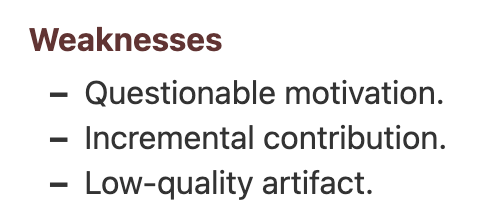
\includegraphics[width=0.9\textwidth]{微信图片_20260810190620_191_105.png}

\subsection{方法要求}

\begin{itemize}
  \item 不增加主模型训练，不依赖新标注或额外幻觉判别模型；最好是一键外接那种。
  \item 只围绕该差异设计一个不可被现有 attention/value/lookahead/verification 直接替代的最小干预；
  \item 在写出 forward-equivalent 成本与最强 related-work kill test 后，才进入最小 pilot。
\end{itemize}

在完成这一步之前，继续生成第 61 个“数学对象加视觉 KV”候选的边际价值很低。按用户停止规则，本档案到 Idea 60 为止，不补做本地实验。

\subsection{RoPE 与历史 KV}

物理移除某些历史视觉 KV 并不必然要求重新计算所有后续 KV。若实现保留每个 cache entry 的原始位置并在 attention 中使用正确位置，剩余 K/V 可以继续使用；真正危险的是把压缩后的物理索引误当成新的序列位置，或改写已经正式生成的文本前缀。当前 VLessHallu 代码将原始位置单独跟踪，并只裁剪视觉 token，文本和已生成 token 不进入删除集合，因此该工程路径与“修改历史文本后整体重算”不同。

简单来说，在causalLM下，你可以禁用前面的kv cache，但不要删除或插入，否则操作区域之后的所有kv cache必须重算。

\section{抽卡自动review标准}

\begin{enumerate}
  \item 第一位 reviewer 为独立 xhigh 5.6 subagent，明确要求不查看记忆，并必须打开工具检索 related work；
  \item 只有第一审严格大于 7，才调用 OpenRouter 的 Gemini 3.1 Pro 与 Grok 4.5，二者均开启 web search；不过我建议gemini换claude，gemini给的分虚高
  \item 三位 reviewer 的分数必须全部严格大于 7，平均分和最高分均不能补偿最低分；
  \item 某一候选失败后才生成下一候选；达到 50 个后停止，后经用户允许借鉴自动科研项目再追加最多 10 个；
  \item 整个方向搜索阶段不运行本地模型实验。
\end{enumerate}

\section{当前 VLessHallu 工程}

主要由gpt实现了四篇参考文献的复现 benchmark。包括baseline、单独方法和聚合方法。结果是散着都很好，放一起分数一般。注意当前放一起是没有任何novelty的，属于incremental contribution的同时，也没有在所有方面有更优结果，特别是CHAIRS-F1。

\clearpage
\part{手动审查后失败的典型idea}

本部分优先记录用户逐步追问、机制拆解和 related-work 查杀过的方向。

结论不只依据初始 novelty 分数，而是考察方法是否符合真实自回归过程、是否被更直接方法支配、是否有足够作用域，以及核心算法能否在不过度增加计算的条件下成立。

后面就是AI自己写的idea和总结了。

\section{Prospective Evidence Coalition KV Control}
\label{sec:pec}

\subsection{原始方案}

Idea 1 的暂定题目为 \emph{Look Before You Ground: Prospective Evidence Coalitions for Training-Free Hallucination Control in MLLMs}。其核心不是预测一个抽象风险分数，而是提前暴露模型将要作出的语义承诺，再通过视觉失明与区域恢复实验寻找能改变该承诺的最小证据 coalition。

设当前正式 cache 为 $C_t$。每隔 $m$ 个真实 token，从 $C_t$ 分叉生成长度为 $h$ 的临时轨迹
\[
\hat y_{t+i}=\arg\max_y p(y\mid C_t,\hat y_{t+1:t+i-1}).
\]
草稿不会提交。固定草稿后，分别在完整视觉 KV 与视觉 null-KV 下 teacher-forced replay。若未来位置 $j$ 的高置信承诺在拿走视觉信息后仍几乎不变，则定义其语言先验风险为
\[
R_j=C_j\exp\left(-\frac{|M_j^{\mathrm{full}}-M_j^{\mathrm{null}}|}{\tau}\right).
\]
从 null-KV 开始分组恢复视觉区域，并求
\[
S^*=\arg\max_S
\sum_jR_jD_{\mathrm{JS}}(p_j^S,p_j^{\mathrm{null}})
-\lambda|S|
-\beta\sum_j(1-R_j)D_{\mathrm{KL}}(p_j^S,p_j^{\mathrm{full}}).
\]
最后丢弃整个预览分支，回到 $C_t$，在正式解码时给 coalition 对应的原始视觉 KV 施加连续门控。因为正式前缀没有被改写，K/V 也不需要按新文本重算；这里的“回滚”只是丢弃临时分支。

直观例子是：模型当前写到“图片中，一名男子正在”，预览分支准备生成“骑着一匹棕色的马”。在 full 与 null replay 中，如果“马”在失明后仍很高，就表明它主要来自语言先验。逐区域恢复时，若人物下方区域使“马”下降而“自行车”上升，则回到正式分支后加强该区域，再让模型重新决定下一个 token。

\subsection{用户质疑一：所谓未来预测只是多步贪心}

用户首先指出，未来轨迹本质上是多步 greedy：同一个模型把将来的 token 提前跑了一遍，却不接受这些 token。这个判断是准确的。方案没有新预测器，future draft 只是一个不提交的 lookahead，类似 speculative decoding 的 draft 阶段，却没有 verifier acceptance 带来的计算复用。

这带来三项问题：

\begin{itemize}
  \item 单条 greedy 轨迹有 tunnel vision，早期一步变化会使后续风险估计整体失效；
  \item full/null 分支并非同时描述真实未来，只是固定同一草稿后的局部对照；
  \item “某区域能改变马的概率”只证明因果影响，不保证它会把输出改成正确的自行车。
\end{itemize}

因此，正确的机制表述应是
\[
\text{未来预览}
\rightarrow
\text{视觉失明测试}
\rightarrow
\text{区域恢复定位}
\rightarrow
\text{回到当前时刻重新生成},
\]
而不是把 future trajectory 本身宣称为创新。

\subsection{用户质疑二：计算量不可接受}

设每 $m=8$ 个正式 token 触发一次探测，lookahead 长度 $h=8$，图像分成 $G=16$ 个区域。一次探测包含：

\begin{itemize}
  \item 未来预览：8 步；
  \item null-visual replay：8 步；
  \item 16 个区域恢复：$16\times 8=128$ 步；
  \item 原本就要执行的正式生成：8 步。
\end{itemize}

总计约为 152 步，相对原本 8 步接近 $19\times$。把区域分支放进 batch 只能改善 wall-clock latency，不能降低总 FLOPs，且会增加显存。

三个表面修补都会让 novelty 消失：

\begin{enumerate}
  \item 用一次反向传播同时估计所有区域影响，成本降到约 2--3 倍，但会接近 LIME 的 inference-time relevance/KV optimization；
  \item 直接使用未来 query attention 排序，成本较低，却退化为 LAQ、MM-ShiftKV 或 PruneHal 一类 future-query/cache scoring；
  \item 接受 preview token 以避免浪费，则变成 speculative decoding，而且危险 token 一旦被接受就来不及提前纠正。
\end{enumerate}

\subsection{最终判断}

Idea 1 的 $8/8.5/8$ 来自旧的无联网 reviewer 协议，只说明完整包装在表面上显得新颖，不能覆盖用户发现的工程否决。该方向最终为 \reject：它以大量反事实分支换取定位精度，不符合“不过度增加推理开销”的硬约束。后续方向不得再次把“多步预览、丢弃、分组遍历、正式重跑”包装成轻量 future-aware 方法。

\section{Hall-Certified Prospective Matching Cache}
\label{sec:hall-cache}

\subsection{原始动机：逐项可信不等于联合可满足}

该方向试图解决一种逐 claim 分数无法表达的错误：多个未来实体声明分别具有较高视觉分数，但它们实际重复使用同一个视觉区域作为证据。设未来短语包含实体槽
\[
C=\{c_1,\ldots,c_m\},
\]
视觉侧包含实例级候选区域
\[
R=\{r_1,\ldots,r_n\},
\]
任意 grounding 前端给出支持矩阵
\[
s_{jr}=\operatorname{GroundScore}(c_j,r).
\]

逐 claim 判断只考察
\[
q_{\mathrm{ind}}=\min_j\max_r s_{jr},
\]
因此允许不同实体槽无限复用同一区域。Hall 版本要求不同实体具有不同视觉见证：
\[
\gamma(C,R)
=
\max_{\pi\ \mathrm{injective}}
\min_j s_{j,\pi(j)}.
\]
恒有 $\gamma(C,R)\le q_{\mathrm{ind}}$。两者之差
\[
\kappa=q_{\mathrm{ind}}-\gamma
\]
是 evidence collision gap，用于刻画“每个声明单独看似可信，但整组声明无法同时成立”。

例如，图中只有一只狗，模型准备生成“两只狗”，支持矩阵为
\[
S=
\begin{bmatrix}
0.93 & 0.08\\
0.91 & 0.07
\end{bmatrix}.
\]
第一列是真狗区域，第二列是草地区域。逐项分数为 $q_{\mathrm{ind}}=0.91$，但单射匹配必须把一个实体分配给草地，因此 $\gamma=0.08$。Hall 方法希望显式暴露这种视觉证据的重复记账。

\subsection{原始算法设计}

\subsubsection{未来实体与视觉实例}

每隔 $L$ 个正式 token，运行长度为 $h$ 的低频 shadow draft，不提交草稿内容，只提取即将出现的实体、数量、属性和关系。数词 $k$ 被展开为 $k$ 个可交换实体槽；属性附着于实体，不额外占用独立区域。例如，“两只棕色狗”形成两个带棕色属性的狗实例，而不是把“棕色”当成第三个实体。

视觉侧不能直接把每个 patch 当作对象。原方案拟对相关视觉 token 的二维位置与响应做局部峰值检测和连通聚类，得到区域集合 $R$。这是方法成立的关键前提：若视觉编码器已经把六根手指压成五个不可分离响应峰，后续匹配无法凭空恢复第六个实例。

\subsubsection{Claim--region 边权}

原始边权为
\[
w_{jr}
=
\sum_{\ell,h}\sum_{i\in r}
a^{\ell h}_{ji}
\left\langle
W_O^{\ell h}v_i,\,
U(c_j)-U(\bar c_j)
\right\rangle,
\]
其中 $a_{ji}^{\ell h}$ 是 future claim 对视觉 token 的 attention，$v_i$ 是 value，$U(c_j)-U(\bar c_j)$ 是 claim 相对竞争语义的输出方向。该定义要求区域既能被 future query 寻址，又确实向 residual stream 写入支持该 claim 的内容。

为了更直观，可拆成
\[
A_{jr}=\sum_{i\in r}a_{ji},
\qquad
\bar v_{jr}=\frac{\sum_{i\in r}a_{ji}v_i}{A_{jr}+\epsilon},
\]
\[
S_{jr}=\left\langle U(c_j)-U(\bar c_j),W_O\bar v_{jr}\right\rangle,
\qquad
w_{jr}=A_{jr}S_{jr}.
\]
其含义是
\[
\text{读了多少}\times\text{读到的内容在支持还是反对什么}.
\]
实际建图时，比直接按乘积排序更稳妥的形式是双条件：
\[
(c_j,r)\in E
\iff
A_{jr}\ge\tau_A
\quad\land\quad
S_{jr}>\tau_S.
\]

该定义形成逐区域贡献账本：
\[
\sum_r w_{jr}
=
\left\langle
U(c_j)-U(\bar c_j),
W_O\sum_i a_{ji}v_i
\right\rangle.
\]
左侧是局部直接语义贡献，右侧是整个视觉 attention output 在目标方向上的写入。它不是完整 causal importance；删除区域后 softmax 会重新归一化，后续层也会改变。

\subsubsection{Hall 证书与最小恢复}

对阈值 $\tau$ 建立二部图
\[
E_\tau=\{(c_j,r):s_{jr}\ge\tau\}.
\]
令 $\nu(G_\tau)$ 为最大匹配大小，则
\[
\delta_\tau
=m-\nu(G_\tau)
=\max_{X\subseteq C}\left(|X|-|N_\tau(X)|\right).
\]
当 $\delta_\tau>0$ 时，不存在让所有未来实体同时获得不同视觉见证的分配。最大化式中的 $X$ 是可解释 Hall witness。实现中不必枚举所有子集：先求最大匹配，再从未匹配实体做一次 alternating-path 搜索即可取得 deficient set。

原方案还考虑逐渐降低 $\tau$，计算最大瓶颈匹配
\[
\tau^\star=\max_M\min_{(c,r)\in M}w_{cr},
\]
以区分“完全不可匹配”与“只能依赖极弱边才能匹配”。

设 $A\subseteq R$ 为 active visual cache 的区域，$R$ 为可恢复的完整视觉区域池。分别计算
\[
\delta_{\mathrm{active}}=m-\nu(G_\tau[C,A]),
\qquad
\delta_{\mathrm{full}}=m-\nu(G_\tau[C,R]).
\]
由此区分：

\begin{enumerate}
  \item $\delta_{\mathrm{active}}=0$：当前 cache 足以支持未来实体；
  \item $\delta_{\mathrm{active}}>0$ 且 $\delta_{\mathrm{full}}=0$：风险由 KV pruning 引起，完整 cache 仍有足够证据；
  \item $\delta_{\mathrm{full}}>0$：完整视觉表示也不能支持未来声明，是内容级 overclaim。
\end{enumerate}

对第二种情况，原方案求
\[
M^\star
=\arg\min_{\substack{M\text{ 为完整匹配}}}
\sum_{(c_j,r)\in M}\mathbf{1}[r\notin A],
\]
即恢复使联合匹配重新可行所需的最少冷区域。例如红狗 claim 与普通狗 claim 都占用 active cache 的红狗区域，而黑狗区域在冷端，则沿
\[
c_{\mathrm{red}}
\rightarrow r_{\mathrm{red}}
\rightarrow c_{\mathrm{dog}}
\rightarrow r_{\mathrm{black}}
\]
恢复黑狗区域并重新分配，而不是为两个 claim 分别做 top-$k$。

更复杂的版本还计划保留最大匹配、最小 Hall-deficit cut 与交替路径交换集中的 KV，并用 transversal matroid 或 capacitated $b$-matching 表述“匹配基及其交换集保持未来可匹配性”。这些保证只对已经构造出的支持图成立，不能反向证明该图忠实反映图像。

\subsection{用户质疑一：六根手指数成五根并非 Hall deficiency}

gpt指出“六根手指的图经常被模型认成五根”是现实对应。人工复核发现，这个例子恰好揭示单向 Hall 的方向性缺陷。

若图中有六个可分视觉实例，而模型只声明五个，则
\[
|C|=5,\qquad |R|=6,\qquad |M|=5.
\]
五个语言槽都能匹配到不同手指，Hall 条件完全满足；未被语言提及的第六根手指不会产生 claim-side deficiency。单向 Hall 能检测的是相反情况：图中只有五根，模型却准备声明六根，此时 $|C|=6>|R|=5$，至少一个语言槽没有独立视觉见证。

若要同时检测漏报，需要加入双向实例核算
\[
d_{\mathrm{over}}=|C|-|M|,
\qquad
d_{\mathrm{omit}}=|R^\star|-|M|,
\]
其中 $R^\star$ 必须是可靠目标实例集合，不能是所有视觉 patch。否则开放式 caption 中未被提及的背景对象会产生大量假阳性。一旦方法必须可靠构造 $R^\star$ 并检查视觉侧覆盖，它就开始直接估计实例总数，迅速退化为比现有 counting 系统更间接的计数方法。

\subsection{用户质疑二：边权是否真的优于 attention}

在没有实验或消融时，不能证明 $w_{jr}$ 会在 benchmark 上优于 attention。能给出的只有信息不足反例：保持 $Q$、$K$ 和 attention 完全不变，只改变某区域的 $V$，区域对 claim 的支持语义已经改变，但任何 attention-only 规则输出不变。因此 attention 不能普遍识别“被读取的区域是在支持还是反对 claim”。

这只证明 attention-only 不充分，并不证明 $A_{jr}S_{jr}$ 最优。它还受到删除后的 softmax 重归一化、后续 MLP/attention 传播、输出方向选择和竞争项 $\bar c_j$ 定义影响。因此 $w_{jr}$ 最多应称为 \emph{local direct semantic contribution}，只能作为可替换边构造器，不能作为核心创新。

只在一个近输出层计算时，额外算术量约为
\[
O(hN_vd_h).
\]
图匹配本身不重。真实开销风险来自 future draft，以及导出 attention 时可能退出 FlashAttention 快速路径。“图算法复杂度低”不等于整套方法低成本。

\subsection{与最相近 counting 工作的比较}

\begin{table}[htbp]
\centering
\footnotesize
\begin{tabularx}{\textwidth}{p{0.17\textwidth}X X p{0.18\textwidth}}
\toprule
工作 & 核心做法 & 与 Hall 的重叠和差异 & 对 Hall 的威胁 \\
\midrule
\href{https://arxiv.org/abs/2605.17826}{CounterCount}
& 构造违反常识数量的图像，如额外手指、耳朵或轮子；提供部件 mask/框，在推理时放大目标视觉 token 并压低背景 attention
& 现象与干预对象最接近。Hall 把数量展开为多个实例槽并要求不同 witness，但 CounterCount 对目标现象更直接
& 很高。若 Hall 最终也是定位部件并增强区域，它只是复杂替代 \\
\addlinespace
\href{https://arxiv.org/abs/2412.00686}{LVLM-COUNT}
& 使用 GroundingDINO、SAM 与分治图像分别计数，避免切分造成重复计数
& 二者都要求实例不可重复消费。Hall 可输出 deficient set 与 active/full cache 差异，但自身不提供可靠实例分割
& 很高。若使用相同检测前端，“一实例只能匹配一次”容易被视为图匹配重述 \\
\addlinespace
\href{https://arxiv.org/abs/2607.09544}{The Count Is There, but Misaligned}
& 训练 count、output-count 与 error probes；高风险时重新提示或 activation steering
& 都在内部提前检测数量错误。该工作给全局错误概率；Hall 可指出具体冲突和恢复区域
& 中高。若 Hall 只是 deficit 触发重生成，它像一个更脆弱的手工 detector \\
\bottomrule
\end{tabularx}
\end{table}

其他相关结果进一步压缩空间：\href{https://arxiv.org/abs/2403.01373}{Quantity Matters} 已定义 number hallucination 并用一致性训练缓解；\href{https://arxiv.org/abs/2604.10039}{Counting to Four Is Still a Chore for VLMs} 指出计数信息可能在视觉投影处较强，却在语言层衰减并受文本先验干扰；\href{https://arxiv.org/abs/2407.06192}{Multi-Object Hallucination} 已验证多对象场景增加幻觉风险。

Hall 尚可守住的窄问题只有
\[
q_{\mathrm{ind}}\ge\tau
\quad\text{但}\quad
\gamma<\tau,
\]
即每个 claim 独立看都有高分证据，但多个 claim 因复用同一实例而无法同时成立。若进一步满足
\[
\gamma_{\mathrm{full}}\ge\tau,
\qquad
\gamma_{\mathrm{active}}<\tau,
\]
则错误可归因于视觉 KV pruning 破坏实例多样性。这是 counting 工作未直接覆盖、也最有辨识度的窄切口。

\subsection{更广 related work 边界}

Hall 的外围组件均位于拥挤赛道：
\begin{itemize}
  \item \href{https://arxiv.org/abs/2505.20334}{LAQ} 与 \href{https://arxiv.org/abs/2603.10899}{LookaheadKV} 已利用 future query/lookahead 管理 KV；
  \item \href{https://arxiv.org/abs/2510.19183}{PruneHal} 与 \href{https://arxiv.org/abs/2602.04268}{KVSmooth} 已直接面向多模态幻觉干预视觉 KV；
  \item \href{https://openaccess.thecvf.com/content/CVPR2026/papers/Wang_Same_Attention_Different_Truths_Put_Logit-Lens_over_Visual_Attention_to_CVPR_2026_paper.pdf}{SADT} 已指出高 attention 不代表 value 真正支持输出词；
  \item \href{https://openreview.net/forum?id=mjHlitXvReu}{VLDet} 等 grounding 工作已使用区域--语言二部匹配。
\end{itemize}

未找到完全等价的“future entity Hall deficit 加 active/full cache 增广恢复”，但 reviewer 很容易将整体概括为
\[
\begin{aligned}
&\text{future lookahead}+\text{region--word matching}\\
&\quad+\text{Hall 后处理}
+\text{hallucination-aware KV restoration}.
\end{aligned}
\]
Hall 定理本身不能证明论文贡献独立于这些前端。

\subsection{最终判断：算法切口独特，但作为方法是下位替代}

正式 novelty 评分为 $8.2/9/7$，不满足三位 reviewer 均严格大于 7。用户的人工结论比 novelty 分数更直接：

\begin{quote}
Hall 是现有计数和局部视觉干预方法的下位替代：算法形式新，但在目标任务上不完整且未必有用。
\end{quote}

淘汰理由为：

\begin{enumerate}
  \item 单向 Hall 能检测 over-count，却不能检测用户给出的典型 under-count；
  \item 加入双向覆盖后与 counting 高度重叠，并在开放 caption 中产生未提及对象假阳性；
  \item 方法依赖视觉编码器先形成稳定实例区域，而这正是手指、相邻物体和细粒度部件中最不可靠的一环；
  \item CounterCount、LVLM-COUNT 与内部 count probe 提供更直接的诊断或修正；
  \item $w_{jr}$ 只是局部语义分解，不能在无消融时证明优于 attention；
\end{enumerate}

因此该方向不应作为主论文继续投入。可保留的仅是诊断思想：\emph{individually plausible claims may compete for the same visual witness}。只有先证明 evidence collision 在 AMBER、CHAIR 或 MMHal-Bench 中高频出现，才值得重新考虑轻量诊断版本。

\section{Future Margin Basis Cache}
\label{sec:fmbc}

\subsection{原始动机与算法}

Future Margin Basis Cache（FMBC）不再给每个视觉 token 一个标量重要度，而试图判断哪些视觉 token 对多个未来词表决策提供不可相互替代的证据方向。

对未来位置 $t$ 的草拟 token $y_t$ 与竞争 token $a$，定义
\[
m_{t,a}=z_t(y_t)-z_t(a).
\]
对视觉 token $i$ 构造贡献向量
\[
c_i=[c_{i,1},c_{i,2},\ldots,c_{i,M}]^\top,
\]
其中 $c_{i,j}$ 是该 token 对第 $j$ 个 future margin 的有符号局部贡献。将这些列组成
\[
C=[c_1,c_2,\ldots,c_{N_v}].
\]

原始算法包含三步：

\begin{enumerate}
  \item 用 rank-revealing QR 或 column subset selection（CSS）选择少数线性独立证据列；
  \item 强制保留无法由正向证据列重构的负向 veto 列；
  \item 用精简 cache 重放 future block，若 margin 误差过大，则补回投影 residual 最大的视觉 token。
\end{enumerate}

直观例子是：两个苹果区域对“苹果”和“红色”的 future margins 提供近似方向，一个低 attention 的空桌面区域独自否决“有杯子”。FMBC 希望保留一个苹果代表和空桌面 veto，而不是两个相似苹果区域。

人工复核前，该方向首审 novelty 为 $7.5$，Grok 搜索复审为 $7$，Gemini 没有返回有效 JSON，因此本来就未满足严格门槛。

\subsection{第一层问题：线性张成不等于保留实际 margin}

即使若干贡献列近似共线，也不能只留其中一列。若一百个弱证据沿同一方向累积，保留一个代表会保留 span，却丢失总 margin mass。删除 token 还会改变 softmax 归一化，使完整 cache 上测得的 $c_i$ 不再适用于精简 cache。

因此原方案至少还要同时约束：

\begin{itemize}
  \item 贡献方向覆盖；
  \item signed margin mass 保真；
  \item reduced-cache replay 后的实际 margin 误差。
\end{itemize}

一旦正确性依赖 reduced-cache verification，RRQR 就不再提供核心保证，只是初始候选启发式。

\subsection{用户的关键反驳：错误地静态化自回归查询}

默认 Transformer attention 并不存在视觉 token top-$k$。在未压缩的基线中，所有可见 KV 都参与 attention；top-$k$ 是某些缓存方法额外施加的选择，或最终词表解码中的候选操作。

更关键的是，“苹果”“红色”和“杯子”对应不同解码时刻：
\[
q_{\mathrm{apple}}\rightarrow A(q_{\mathrm{apple}},K,V),
\]
\[
q_{\mathrm{red}}\rightarrow A(q_{\mathrm{red}},K,V),
\]
\[
q_{\mathrm{cup}}\rightarrow A(q_{\mathrm{cup}},K,V).
\]
三个 query 来自不同前缀，具有不同 hidden state 与 softmax 分母。模型生成到“苹果”时自然读取对象证据，生成到“红色”时再读取颜色证据。FMBC 却把它们写成同一静态列
\[
c_i=
[c_i^{\mathrm{apple}},
c_i^{\mathrm{red}},
c_i^{\mathrm{cup}}]^\top
\]
并据此判断视觉 KV 是否线性可替代。

该线性相关性不代表真实解码中的可替代性。如果第一步把“苹果”改成“梨”，后续“红色”和“杯子”的 query 都会随前缀变化。因此一条 greedy trajectory 上的多个局部 margin 不是同时成立的固定坐标。

“红苹果”作为单一词表 token 也不能挽救方法：

\begin{itemize}
  \item 若只有一个当前 margin，basis selection 退化成标量贡献排序；
  \item 区域内均匀 attention 可能正是聚合颜色与对象信息所需，不能只留一个线性代表；
  \item 若进一步合并相似视觉 token，则退化为普通 visual-token merging。
\end{itemize}

若修正为“取得每个 future query，再保留各时刻所需视觉 token 的并集，并在用后释放”，basis 部分会变得多余，整体退化为拥挤的 future-attention/lookahead cache scheduling。

\subsection{第二层问题：signed veto 与 RRQR 不匹配}

一个视觉 token 可能对“苹果相对梨”为正，却对“有杯子相对无杯子”为负，因此没有稳定的全局 positive/veto 划分。普通 RRQR 允许
\[
c_i\approx\sum_{j\in B}\alpha_jc_j,
\qquad \alpha_j\in\mathbb{R},
\]
而真实 attention 聚合使用非负、归一化且随 query 改变的权重。“在线性 span 中可重构”不等于“在 attention 中可替代”。若要保持实际语义，应改为逐自回归状态的 convex/conic covering；但这样一改，普通 RRQR 又不适用。

FMBC 因而存在两个互相强化的错误：

\begin{enumerate}
  \item 自回归时序被压成静态 future-margin 空间；
  \item 静态空间内部采用不符合 attention 非负归一化结构的线性重构。
\end{enumerate}

\subsection{机制级 related-work 查杀}

\begin{table}[htbp]
\centering
\footnotesize
\begin{tabularx}{\textwidth}{p{0.20\textwidth}X p{0.20\textwidth}}
\toprule
FMBC 组件及最近工作 & 已有机制 & 重叠判断 \\
\midrule
RRQR/CSS：\href{https://arxiv.org/abs/2606.18681}{SPARE}
& 将 visual-token pruning 写成 CSSP，使用 RRQR、Gram--Schmidt 与最大投影 residual 逐列选择
& 几乎直接重叠 \\
\addlinespace
条件化子空间：\href{https://arxiv.org/abs/2603.21105}{ResPrune}
& text-conditioned subspace reconstruction，每轮加入 residual energy 最大的视觉 token
& 直接重叠 \\
\addlinespace
输出敏感度：\href{https://aim-skku.github.io/ZOO-Prune/}{ZOO-Prune}
& 通过扰动估计视觉 token 对输出的 sensitivity，并结合 diversity
& 信号和目标层面重叠 \\
\addlinespace
互补证据：\href{https://arxiv.org/abs/2606.18681}{SPARE}，\href{https://arxiv.org/abs/2607.07033}{AnchorPrune}
& anti-relevance，或 relevance anchor 加 complementary context
& 与 veto/互补证据概念重叠 \\
\addlinespace
语义支持：\href{https://openaccess.thecvf.com/content/CVPR2026/papers/Wang_Same_Attention_Different_Truths_Put_Logit-Lens_over_Visual_Attention_to_CVPR_2026_paper.pdf}{SADT}
& 用 logit lens 判断高 attention 区域的 value 是否支持输出词
& 语义诊断直接相邻 \\
\addlinespace
负视觉信号：\href{https://arxiv.org/abs/2603.10360}{One Token, Two Fates}
& 把被裁视觉 token 构造成 latent negative sample
& 反证思想重叠 \\
\addlinespace
压缩后验证：\href{https://arxiv.org/abs/2605.17613}{VeriCache}
& 用压缩 cache 草拟并由完整 cache 验证
& 验证闭环重叠 \\
\bottomrule
\end{tabularx}
\end{table}

没有检索到一篇论文完整复制“future-margin matrix、signed veto、RRQR/CSS、重放补 residual”这一整套组合。但组合不等于独立核心创新：
\[
\text{conditioned matrix}
+\text{RRQR/CSS}
+\text{residual greedy}
\]
已经与 SPARE 和 ResPrune 高度一致。把输入从视觉 embedding 换成 future-margin attribution，更可能被视为目标矩阵替换；重放验证又与 VeriCache 相邻。

唯一表面未被完整覆盖的是“在 future-margin contribution matrix 上构造有符号锥，保留不能被支持列替代的 veto 列”。但该部分同时受到自回归静态化与 attention 非负归一化问题影响，尚不是定义稳定的新原理。

\subsection{最终判断}

FMBC 的问题不是少一个正则项，而是核心抽象不符合自回归解码：

\begin{quote}
不同时间、不同前缀下的未来 margin 不能被无条件视为固定线性证据空间；修正这一点后，basis selection 的核心 novelty 随之消失。
\end{quote}

综合查重后，严格 novelty 应从初始 $7.5$ 下调到约 $5$--$6$。该方向最终为 \reject，且不应再以“换矩阵、换分解方法”的形式重新包装。

\clearpage
\part{总结}

\section{反复出现的错误}

\subsection{成熟算法超级大聚合}

Hall、Rado/matroid、zonotope、Farkas separation、EVT、permutation test、CSP、sheaf、network flow、SPRT、set cover、minimax/double oracle、delta debugging、causal mediation 和 CEGAR 都能生成清晰算法。但 reviewer 的共同判断是：若问题的核心经验现象没有自然要求这个算法，方法就会被视为“成熟算法迁移到 visual KV”，而不是视觉幻觉中的新原理。

\subsection{切入似乎很对，实际非常狭隘}

以下推理均不成立：
\[
\text{局部 attention output 保真}
\not\Rightarrow
\text{最终回答正确},
\]
\[
\text{支持图存在完整匹配}
\not\Rightarrow
\text{图像中真的有对应实例},
\]
\[
\text{future draft 上 cache 等价}
\not\Rightarrow
\text{真实后续前缀上仍等价}.
\]

\subsection{多步预测在自回归生成模式下的严谨性问题}

很多候选将当前层的 attention、value-to-logit contribution 或固定 draft 轨迹当成未来的稳定对象。但自回归改变早期 token 后会改变所有后续 query。若未来状态真的已被完整跑出，方法又要解释为什么不直接使用这些 query，并证明额外 replay 可被摊销。

\section{采用自动科研提示词, 追加十轮}

从开源自动科研系统抽取搜索与反驳结构。

\paragraph{IDEAgent。}
参考 \url{https://github.com/declare-lab/IDEAgent} 的 quality-diversity 搜索，把候选按
\[
\begin{aligned}
(&\text{failure mode},\text{diagnosis},\text{signal},\text{intervention},\\
 &\text{locus},\text{objective},\text{evaluation},\text{relaxed assumption})
\end{aligned}
\]
建立语义签名；分别维护 literature archive、accepted/rejected idea archive 与 ancestor chain。探索与改进分离，并禁止简单组合、换名和把已有模块搬到新任务。

\paragraph{Heuresis。}
参考 \url{https://github.com/a-antoniades/Heuresis} 的 MAP-Elites cell-targeted ideation。某一语义 cell 拥挤时，不继续调参数，而要求改变 load-bearing mechanism；每个 idea 必须给出 executable contract、最小 falsifier、强基线和失败攻击。其局限也被保留：quality-diversity 能扩大覆盖，不保证扩大 novelty frontier。

\paragraph{AI Scientist v1/v2。}
参考 \url{https://github.com/SakanaAI/AI-Scientist} 与 \url{https://github.com/SakanaAI/AI-Scientist-v2}。对每个候选依次搜索 exact phrase、机制同义词、相同任务、相同实验设计和不同术语下的近邻，并明确写出“最可能杀死 novelty 的工作”；检索结果必须回流到 idea revision。

\paragraph{CodeScientist。}
参考 \url{https://github.com/allenai/codescientist} 的 paper--code 联合搜索。候选必须列出可证伪假设、对照组、主要指标、强基线、最小 pilot、依赖项、工作量与放弃条件。本任务没有运行 pilot，但用这些 executable-contract 约束排除了只能提供漂亮数学叙述的候选。

\paragraph{ResearchAgent 与 Agent Laboratory。}
参考 \url{https://github.com/JinheonBaek/ResearchAgent} 的 Problem--Method--Experiment 分解，为 novelty、feasibility 与 utility 分别审查；低分轴不能由其他高分项平均补偿。Agent Laboratory 的启发是让具体否决理由回流到方法与实验定义。

\paragraph{最终合成提示。}
追加十轮采用以下约束：

\begin{enumerate}
  \item 先列语义签名和最接近的已拒绝祖先；
  \item 写出唯一 load-bearing mechanism，不允许若干已有模块并列；
  \item 指定最可能杀死 novelty 的 related work 并做机制级差分；
  \item 给出核心经验现象、可证伪预测、强控制组与计算预算；
  \item reviewer 主动执行 exact、mechanism、task、evaluation 与 synonym 五类检索；
  \item 使用三审合取门槛，由最低分而非平均分决定通过；
  \item 赛道拥挤时下一轮必须换因果对象或干预原语，不继续修饰上一方案。
\end{enumerate}

该流程产生 causal intervention、sequential testing、signed multicover、minimax、behavioral predicate search 与 cross-modal handoff 等不同候选，但也支持 \emph{AI Research Agents Narrow Scientific Exploration}（\url{https://arxiv.org/abs/2605.27905}）的警告：自动科研系统容易把成熟算法迁移到新对象，并把“组合罕见”误认为“领域原理新颖”。

结果：

| Idea | 方法 | 分数 | 失败原因 |
|---|---|---:|---|
| 51 | VisPF | 4 | query-aware page retrieval 与决策证书已有强近邻 |
| 52 | MKVC | 5 | K/V permutation 更像昂贵诊断，且 exchangeability 不成立 |
| 53 | FMBC | 7.5 / 无效 / 7 | Grok 仅为 7；RRQR、residual add-back、full-cache verification 分别与 SPARE、ResPrune、VeriCache 重叠 |
| 54 | CEGAR-VKV | 7.5 / 8 / 3 | Grok 判定只是把 CEGAR 模板迁移到 KV cache，且需要反复 replay |
| 55 | PairGuard-KV | 6 | `2×2` 成对干预成本高，与 interaction attribution 接近 |
| 56 | LeaseSPRT-KV | 5 | 通用 SPRT 迁移，paired replay 昂贵，自回归观测也不满足简单 i.i.d. |
| 57 | WitnessCover-KV | 4.5 | 本质是 signed future claims 上的 set-cover |
| 58 | MinimaxKV | 3.5 | 通用 minimax/double-oracle 迁移，计算重且未必改善平均指标 |
| 59 | DeltaKV | 3 | 直接迁移 `ddmin`，非单调且只对冻结轨迹成立 |
| 60 | RelayKV | 5 | causal mediation/视觉到文本的信息接管已有近邻，并需多次干预 |

也就那样，53看着高。但还是被否决了，因为它与 SPARE、conditioned subspace/residual greedy 与 ResPrune、full-cache verification 与 VeriCache 直接重叠，因此淘汰。堆得多罢了...效果还不知道呢

\clearpage
\part{完整Idea 1--60摘要}

把这一段复制给gpt就能生成完整方法了，如果你想看某个点完整版的话。全在这里放不太现实。

\paragraph{Idea 1：Prospective Evidence Coalition KV Control。}
每隔若干正式 token 生成短 future draft，对同一草稿分别做 full-visual-KV 与 null-visual-KV replay；从 null cache 分组恢复视觉区域，寻找能改变高风险未来承诺的最小 evidence coalition，再回滚草稿并门控正式分支 KV。评分为 $8/8.5/8$（旧协议）。用户手审指出它本质是“不提交的多步 greedy lookahead”，再叠加 full/null replay 与区域恢复，约 $19\times$ 推理成本；高分作废。

\paragraph{Idea 2：Rejection-Credit Speculative Grounding（RCSG）。}
稀疏视觉 drafter 与完整视觉 verifier 做 self-speculative decoding；首个 rejection $(y^-,y^+)$ 被当作语言先验近邻反事实，并以
\[
c_i=a_i\left\langle W_OV_i,u(y^+)-u(y^-)\right\rangle
\]
形成视觉纠错 credit ledger，随后给原视觉 KV 加有界 attention bias。评分 $7.4/9/6$。Grok 将“视觉受限 drafter 加 dense verifier”视为已有 MLLM speculative decoding 近邻，rejection credit 不足以形成新范式。

\paragraph{Idea 3：Future Decision-Certificate Cache（FDCC）。}
用 block/tree speculative decoding 获得未来分支；把每个未来 grounded token 相对语言先验竞争项的 signed visual margin contribution 组成约束族，求同时保持整棵未来决策树 margin 的最小视觉 KV coreset。评分 $7.4/9/5$。本质仍接近 future-query/lookahead KV selection 加 margin-preserving coreset，树草稿与优化成本也偏重。

\paragraph{Idea 4：Hadamard-Coded Causal Masking（工作标签）。}
用 Hadamard/随机编码的成组视觉 mask，在少数 multiplexed 测量中恢复各视觉区域对 future logit margin 的因果贡献，以避免逐区域 forward。评分 $5.8$/未触发/未触发。编码 mask、group testing 与 compressed-sensing attribution 均有充分近邻，只是把通用归因迁移到视觉 KV。

\paragraph{Idea 5：Kinetic Evidence Frontier（工作标签）。}
不直接生成 future token，而由最近 query 的运动估计未来 query 可达区；把视觉 key 看作线性函数，保留可能进入未来 attention 上包络或改变 signed evidence boundary 的 KV。评分 $5.8$/未触发/未触发。与 Foresight、future-query cache prediction 和几何 MIPS/upper-envelope 接近；query 轨迹假设与 softmax 误差界不稳。

\paragraph{Idea 6：SEW-KV（工作标签）。}
对视觉块做自适应 Monte-Carlo/importance sampling，以序贯置信区间判断稀疏 cache 是否已足够近似完整 attention 或 future margin；证书未收敛时继续恢复块。评分 $5.8$/未触发/未触发。与自适应稀疏 attention、PAC/Monte-Carlo attention approximation 高度重合，幻觉部分主要是应用替换。

\paragraph{Idea 7：Hall-Certified Prospective Matching Cache（HPMC）。}
将 future claims 与视觉区域构成带容量二部图；若某 claim 子集 $C'$ 满足 $|N(C')|<|C'|$，则 Hall deficit 指出多个声明重复借用同一视觉证据。保留最大匹配、最小 deficit cut 与 alternating-path exchange set 中的 KV，并沿增广路径恢复冷区域。评分 $8.2/9/7$，因第三审等于 7 而失败。用户进一步指出它无法直接检测“六根手指说成五根”，且是现有 counting/局部干预的下位替代。

\paragraph{Idea 8：Future Signed Heavy-Hitter Cache（工作标签）。}
对多个 future query 的 $QK\times$ signed value-to-logit contribution 做 CountSketch/重频项恢复，寻找未来持续支持或否决 claim 的视觉 KV，而不扫描全部 token。评分 $6.6$/未触发/未触发。CountSketch/MIPS heavy hitters 与 future-query KV recall 近邻很强，signed contribution 只是 scoring signal 变化。

\paragraph{Idea 9：Extreme-Witness Future Cache（EWFC）。}
将“在大量 patch 中取最大证据”视为多重比较偏差；对 future claim 的 signed grounding score 做空间去簇、POT/GPD 极值尾拟合和 extremal-index 校准，再以 e-BH/alpha-investing 控制 future-window FDR。只保留显著正/负极值簇与尾估计边界样本。评分 $8/8/6$。最终被视为把通用 EVT/e-value 校准迁移到视觉 patch evidence，KV 动作仍是阈值保留/恢复。

\paragraph{Idea 10：Permutation-Certified Binding Cache（PCBC）。}
固定 future query 的 attention 权重多重集与 value semantic score 多重集，通过空间块 permutation 检验真实 K--V 配对是否比随机重配更支持 claim；以
\[
(\alpha_i-\bar\alpha)(x_i-\bar x)
\]
的 pivotality 保留正见证、负反证与检验边界 token。评分 $7.2/9/7$。第三审等于 7；更像 causal attribution/permutation test 的新检验，不是新 KV 管理原理。

\paragraph{Idea 11：Zonotope-Separated Future Cache（ZSFC）。}
将每个视觉区域对 $h$ 个 future claim 的 signed correction 写成列 $c_i\in\mathbb R^h$，所有可逆 gate 的可达修正组成 zonotope；若目标 margin 向量在误差盒扩张后的 zonotope 外，Farkas separating hyperplane 给出联合不可救证书，再以 column generation 恢复 reduced-cost 最大的 KV。评分 $7.8/9/7$。线性化与 softmax renormalization 无法覆盖真实 decoder 非线性，整体也像 LP/column-generation 移植。

\paragraph{Idea 12：HALO: Hallucination-Aware Logic Oracle。}
将未来对象、属性、关系声明与视觉候选写成 CSP/factor graph，通过 arc consistency、all-different constraint 与 minimal unsat core 定位联合不可满足声明，再据候选域恢复视觉 KV。评分 $4.8$/未触发/未触发。scene-graph grounding、CSVG/CSP 与 unsat-core reasoning 都有直接近邻，KV 管理只是符号诊断后的附加动作。

\paragraph{Idea 13：Sheaf-Laplacian Obstruction Cache（工作标签）。}
把跨 claim、区域和层的局部证据视为 cellular-sheaf sections，以 sheaf Laplacian 能量或 cohomology obstruction 定位不能拼成 global section 的未来声明，并按有效电阻或谱 leverage 保留视觉 KV。评分 $5.2$/未触发/未触发。Transformer 张量未证明满足所借 sheaf 结构；去掉拓扑术语后仍是图一致性检测加谱 token pruning。

\paragraph{Idea 14：Proof-Carrying Evidence Flow Cache（工作标签）。}
将视觉证据到多个 future claims 的传播写成多商品流；min-cut 或 flow infeasibility 充当 hallucination certificate，cache 保留 terminal cut sparsifier、瓶颈边与恢复可行性所需 KV。评分 $4.7$/未触发/未触发。attention-flow attribution 与 graph cut 已有工作，将 attention 当守恒流并把流可行性等同 semantic grounding 缺乏基础。

\paragraph{Idea 15：Query-Addressable Counter-Witness Cache。}
为未来高风险 claim 构造 synthetic KV dipoles：key 分别沿 $\pm\hat q_j$ 偏移，value 分别写入 claim 的负/正语义方向；校准后只对目标 query 下调幻觉 margin，对近正交 query 一阶抵消。评分 $6.2$/未触发/未触发。synthetic KV、activation steering 与 absence evidence 均有近邻；任意 KV 注入的 off-target 稳定性不足。

\paragraph{Idea 16：Future Visual Controllability。}
用短 draft 构造文本 echo 的严格下三角矩阵 $F$、有限时域增益 $G=(I-F)^{-1}$ 与视觉控制矩阵 $B$；在保持当前 next-token attention output 不变的 null space 中，求最小范数视觉 $V$ 编辑以压制未来文本自激励模式。评分 $4.3$/未触发/未触发。与 cache/activation steering、closed-form editing 接近；局部末层线性化与未来可控性均不稳。

\paragraph{Idea 17：Visual Evidence Ledger。}
联合分配多个 future claims 到视觉 token，并惩罚语义无关 claims 重复消费同一证据；优化后用最小范数 key edit 实现目标路由，同时保持每个 future query 的视觉 partition mass。评分 $5.7$/未触发/未触发。本质接近 OT/coverage/diversity-aware attention routing；“同一 token 不应被多个 claim 共享”对对象、属性、关系并不普遍成立。

\paragraph{Idea 18：TubeCert-KV: Robust Query-Tube Certificate。}
由历史 draft 误差构造未来 query 椭球，对每个视觉 key 求闭式上下界，并把 signed value evidence 合成为整个 query tube 上的 margin interval；按最坏情况恢复 support/veto token。评分 $4.1$/未触发/未触发。robust attention、ellipsoidal bound 与 certified token pruning 已覆盖主干；证书仅保护局部 direct-contribution surrogate，且界可能过松。

\paragraph{Idea 19：Text--Visual Twin / Evidence-Lineage Cache（工作标签）。}
沿 draft 中 attention/value direct-logit contribution 追踪视觉证据如何经 text relay token 传播；future claim 若只剩文本副本而原始视觉 lineage 坍塌，则 pin 或恢复源视觉 KV。评分 $5.7$/未触发/未触发。attention rollout、ALTI-Logit、circuit tracing 与视觉 relay 已覆盖大部机制，lineage 驱动 cache 是组合扩展。

\paragraph{Idea 20：Future Visual Experiment Cache（F-VEX）。}
把 future semantic alternatives 当作多假设检验，把视觉 KV 当传感器；选择使最弱候选对 Chernoff information 最大的 KV 集，以保留最能区分 claim 与竞争项的视觉反证。评分 $4.3$/未触发/未触发。属于经典 sensor selection/active hypothesis testing 迁移；Chernoff 可加性及从 attention/value 得到可靠 likelihood 的假设不成立。

\paragraph{Idea 21：Counterfactual Attention Shield（工作标签）。}
用删除单个/分组 KV 后 softmax numerator 与 denominator 的闭式更新，估计每个 future claim 的精确局部删除效应；保护删除后会放大可疑 claim 的 counter-evidence/sink，淘汰安全项。评分 $4.2$/未触发/未触发。attention token ablation、closed-form deletion、semantic sink 与 output attribution 已有近邻，仍是更精确 importance score。

\paragraph{Idea 22：VetoKV。}
为 future claim 与语义替代项计算 signed visual value-to-logit contribution，专门保留或恢复反对高语言先验 claim 的低-attention veto KV，而不只保留正证据。评分 $6.7$/未触发/未触发，是未进入复审者中的最高分。但 SADT、negative visual evidence、contrastive hallucination mitigation 与 output-aware KV 已覆盖主要动机。

\paragraph{Idea 23：Visual Round-Trip Cache。}
构造 claim $\rightarrow$ region $\rightarrow$ claim 的冻结转移：key 负责寻址，value 经 unembedding 解码回候选词；保留形成正确自返回或导向关键替代词的 patch，删除“key 看似相关但 value 语义不闭环”的视觉项。评分 $5.6$/未触发/未触发。与 SADT 的 value semantic checking、VGA 与 OBCache 的 K/V 联合重要性重叠，round-trip 是评分重写。

\paragraph{Idea 24：Future Claim-Sufficient Two-Tier KV。}
对 future query span $B_Q$ 与 claim-contrast span $B_U$ 保存每个区域的低维 guard statistics
\[
\hat k_i=B_Q^\top k_i,\qquad \hat v_i=B_U^\top v_i,
\]
再由 guard tier 按需将 dormant full KV 提升到 active tier。评分 $3.4$/未触发/未触发。与低秩 KV、query-specific projection、ResKV/ThinK 重合；“充分”只对固定 lookahead subspace 成立。

\paragraph{Idea 25：Rado-Certified Matching Cache（工作标签）。}
把 Hall 的“不同 claim 需要不同区域”推广为 Rado/matroid independent representatives：不同 future claims 不仅匹配不同区域，所选证据还必须在语义贡献空间中线性或拟阵独立；保留 basis 与 exchange candidates。评分 $4.1$/未触发/未触发。数学定理迁移明显，claim、区域与向量独立性的语义对应缺乏依据。

\paragraph{Idea 26：Exact Spatial Jackknife KV。}
一次累计每个空间块的 softmax 分母质量 $Z_{jB}$ 与 value 分子 $N_{jB}$，用
\[
o_{j,-B}=\frac{N_j-N_{jB}}{Z_j-Z_{jB}}
\]
精确得到删除块后的 attention output，无需区域 forward；沿 future claim margin 方向得到 signed leverage 并决定 pin/prune。评分 $3.3$/未触发/未触发。与 CAOTE/closed-form attention ablation 接近，创新主要是把 current token 换成 future claim 与空间组。

\paragraph{Idea 27：Claim-Deadline Visual KV。}
将 future contribution sequence 编译为每个视觉区域的一个或多个需要区间，运行时执行 \texttt{activate(i,s-$\Delta$)} 与 \texttt{deactivate(i,e)}；原始 KV 留在 dormant pool，轨迹偏离时重编译后续生命周期。评分 $4.4$/未触发/未触发。与 cache prefetch、TTL/lifetime scheduling、LAQ/Expected Attention 的未来重要性预测同构。

\paragraph{Idea 28：BalanceKV（reviewer 工作标签）。}
将视觉 token 对 future margins 的正、负向贡献视作 signed vectors，以 discrepancy/vector-balancing 选择小 coreset，分别保存 support mass 与 veto mass，并用 dual witness 判断预算不足。评分 $2.2$/未触发/未触发。属于标准 discrepancy/coreset 迁移；softmax 非线性与 token 依赖破坏向量可加性。

\paragraph{Idea 29：Antisymmetric Relation-Edge Cache（ARE-KV；也出现 FCSGG 标签）。}
在视觉图有向边 $i\to j$ 上构造
\[
K_e=(K_j-K_i)/\sqrt2,\qquad
V_e=(V_j-V_i)/\sqrt2,
\]
用 future relation flow 判断方向一致性，并在风险 span 懒加载 edge read，使关系本身成为可寻址 KV。评分 $4.1$/未触发/未触发。EdgeConv、scene-graph relation feature 与 relation-sensitive head 已有近邻，差分边 cache 是昂贵的工程表示扩展。

\paragraph{Idea 30：GQA Physical-Pool / Per-Q-Head Logical-View Split。}
每个 KV head 只保留一份物理视觉池，但为共享它的每个 query head 建立独立 sparse index view；future draft 决定各 Q-head 可见的视觉地址，避免对象、属性、关系 head 争用统一剪枝集合。评分 $4.5$/未触发/未触发。与 Quest、MagicPIG、per-query sparse attention 和 GQA-aware KV indexing 接近，更像高效 attention 系统设计而非新 hallucination 原理。

\paragraph{Idea 31：Dual-Channel Witness Run Break。}
对短 future draft 中的每个视觉 token，分别用固定随机超平面计算 query--key 地址一致位和 residual--value 语义一致位；两类比特同时成立才记一次命中。以跨 future step 的最长连续命中游程作为视觉见证，并用 Bernoulli run 的有限状态递推设置阈值。首审 $3.4$。SimHash/LSH、future-query cache selection 与游程检验均有成熟来源；独立、正交且同分布零假设也不符合真实 attention。

\paragraph{Idea 32：视觉 attention 剂量--反应边界（正式名称未恢复）。}
沿视觉 attention logit 缩放系数构造连续干预路径，观察 future draft 候选词 margin 随强度的曲线；以过零点、临界剂量或灵敏度管理视觉 KV。首审 $4.1$。attention boosting 与温度缩放已拥挤，softmax 下 margin 对缩放不保证单调，根不存在或多根时定义不稳。

\paragraph{Idea 33：提交式 draft 槽位视觉 KV 嫁接。}
在已提交短 draft 中寻找视觉接收弱、却会被后续 token 高频访问的功能词或标点槽；将真实视觉 token 的完整 KV 经精确 RoPE 迁移后复制到该槽某个 GQA group，使其成为靠近解码尾部的视觉 relay。首审 $4.6$。KV 搬移、cache splice、视觉记忆再注入与 anchor token 已有近邻；覆盖功能词 KV 还可能破坏语言语义。

\paragraph{Idea 34：RoPE 相位锁失效事件。}
将 RoPE 维对写成复数并移除已知相对位置旋转，测量 future queries 与视觉块之间的内容相位合成长度；若 active blocks 均不能形成稳定 phase lock，则恢复越阈冷块。首审 $2.8$。RoPE 相位分析、位置重绑定与 future-query retrieval 已存在，“真实视觉证据必形成跨 token 锁相”也没有机制依据。

\paragraph{Idea 35：视觉证据负债越界事件。}
比较每个 future step 中视觉 attention write 与文本 attention write 对 residual innovation 的对齐，累积为 e-process；最大值越过 Ville 阈值时，解释为 draft 持续转向语言先验，并恢复最能解除越界的视觉块。首审 $3.5$。接近 M3ID/PAS 类视觉依赖衰减指标，只是增加 anytime-valid 统计；条件均值假设无法从冻结 VLM 保证。

\paragraph{Idea 36：视觉码长倒置事件。}
把 future residual innovation 随机投影到低维，分别由视觉 write 与文本 write 构造逐步 Student-$t$ 预测码；若视觉码长显著更大，则认为语言通道更能解释未来，并恢复最能缩短视觉码长的 KV。首审 $4.1$。prequential/MDL、视觉--文本依赖比较与 future draft 都是已有工具，拟合码长也不是真实生成似然。

\paragraph{Idea 37：视觉响应球形化事件。}
收集 future steps 与 attention heads 的单位视觉 write，计算二阶矩阵与球面对称矩阵 $I/r$ 的距离；响应近似各向同性时恢复能产生方向性 spike 的冷块。首审 $2.6$。DSCR 已把视觉 key 各向同性与幻觉联系起来，从 query-conditioned write 球形化到内容幻觉仍缺可靠因果链。

\paragraph{Idea 38：中心--周边差分视觉 KV（正式名称未恢复）。}
以视觉 patch 为中心、空间邻域为 surround，构造类似 lateral inhibition/unsharp masking 的正负 attention/write 对；只有 future claim 的中心支持超过邻域干扰才保留。首审 $2.5$。Differential Transformer、attention-space contrastive guidance、局部--全局解码与 DSCR/KVSmooth 都有近邻；固定邻域也不等于对象边界。

\paragraph{Idea 39：多图像证据银行与 Viterbi 路径（正式名称未恢复）。}
将不同图像/视图的视觉 KV 分组，先做 image-level grouped softmax，再在 future claim 序列上用带切换代价的 Viterbi path 选择持续一致的证据银行，防止实体描述跨图片漂移。首审 $3.0$。grouped/hierarchical attention、多图路由与 structured attention 已有大量工作，且与单图 CHAIR/AMBER 主场景不对齐。

\paragraph{Idea 40：Future-Driven Visual-KV Bitplane Tiering。}
视觉 KV page 由低比特 base 和可挂接 residual bitplanes 组成。future draft 持续使用的 page 恢复高位残差，未使用 page 卸下残差，在固定显存预算下切换 INT2、INT8 或近 BF16。首审 $4.8$。mixed-precision KV、progressive residual quantization、CONF-KV、QuantSpec 与 VeriCache 近邻很强，也缺少“视觉 KV 量化是幻觉主因”的现象。

\paragraph{Idea 41：地址--语义--空间三阶绑定检验（正式名称未恢复）。}
通过受约束的视觉 K/V/位置置换，试图在保留两两边际的同时破坏 query--key 地址、value 语义与空间位置的三阶绑定；future claim 仅在原三元绑定下成立时保留对应 KV。首审 $3.0$。SADT 已检查 attention/value 语义一致性，K/V shuffle 也是常见消融；同时保持所有两两边际的置换通常不可执行。

\paragraph{Idea 42：Time-Unrolled Hall Matching。}
把 future draft 中同一实体的多次提及展开为时间节点，以外观、空间与语义一致性边连接区域，在 time-unrolled graph 上做 matching/min-cost flow；后续属性通过 identity switch 借另一对象证据时产生 deficiency。首审 $3.2$。它是 Hall matching 的扩展，与多目标跟踪、视觉共指和全局 phrase grounding 重叠，且未修复 Hall 边不可靠与作用域窄的问题。

\paragraph{Idea 43：Post-Selection Calibrated Extreme Visual Witness（正式名称未恢复）。}
不直接相信 attention 最大 patch，而把最大值当作 post-selection statistic；用 EVT、Gaussian random-field peak 或 spatial scan statistic 校准局部峰/盆地显著性。首审 $3.0$。校正 winner's curse 只能证明峰值异常，不能证明 patch 语义支持 claim，仍是校准后的 attention top-$k$。

\paragraph{Idea 44：Visual Innovation Cache。}
估计文本 KV 或语言先验张成的子空间，将视觉 value/write 投影到其正交补，只保存不能由文本子空间解释的 innovation residual；future draft 需要某创新方向时恢复对应 KV。首审 $3.0$。ACG、HulluEdit、ResPrune 与 SPARE 已使用视觉--文本正交分解或条件子空间重构；正交于文本不等于视觉真实。

\paragraph{Idea 45：Coded Visual-Provenance Receipt。}
向视觉 KV 或 attention write 注入相互正交的 Hadamard/随机小扰动，再从 future hidden states 用 matched filter 解码“回执”，用少量 forward 判断哪些视觉 token 确实传播到 future claim。首审 $3.2$。activation patching、coded perturbation、zeroth-order attribution 与 HalluTrace 已覆盖主要组成；标签注入会改变被测网络，多层非线性后也无法干净解码因果来源。

\paragraph{Idea 46：Future Head-Coalition Cache。}
在末若干层对视觉 attention heads 做单头和成对开关的 $2\times2$ factorial intervention，以 difference-in-differences 测量 head synergy 对 future claim margin 的作用，再把视觉 KV 预算分配给反幻觉 coalition。首审 $4.4$。head ablation、path patching、Shapley interaction 与 hallucination heads 已成熟；成对实验随 head 数增长过快。

\paragraph{Idea 47：K-Indexed V Materialization。}
保留低比特/摘要 key 作为常驻索引，把昂贵 value 放冷端；future query 先扫描 key，只为可能提供 support/veto 的位置 materialize values。首审 $2.0$。ShadowKV、RetrievalAttention、InfiniGen 与 SpeCache 已广泛研究 key 常驻、value offload 和 query-aware prefetch；加入幻觉语义只是任务迁移。

\paragraph{Idea 48：Non-Monotone Layerwise Visual-KV Re-entry。}
早层剪掉的 layer-local 原始视觉 KV 存在冷池，future query 可让某 patch 在中层缺席、深层重新进入；恢复冷页时同步解除无用热页以保持预算。首审 $1.8$。PLPHP、IdleViT、HAE、HybridKV 与 token recovery/re-entry 已覆盖近乎相同的层间非单调性。

\paragraph{Idea 49：Predictive-Equivalence/Bisimulation KV Merging。}
把视觉 KV 看作对 future queries 产生 attention/output 行为的状态；若两个 token 在当前 draft query set 上不可区分，则合并为同一等价类；出现可区分 future trace 时按 CEGAR/partition refinement 拆分。首审 $2.8$。query-aware KV merging、Attention Matching、KVSculpt 与 predictive-state abstraction 已提供骨架；有限 draft 等价不能保证后续 prefix 下等价。

\paragraph{Idea 50：Integral Evidence Polytope / Projective-Softmax Certificate。}
把每个视觉 token 对 future claim margin 的 softmax numerator/denominator contribution 做齐次提升，在固定预算下用 LP/MILP 选子集；以 Farkas 型不可行证书说明某 claim margin 不能保持。首审 $2.5$。attention coreset、Expected Attention、CAOTE 与 certified KV compression 已覆盖目标；softmax、多层反馈和整数选择使所谓精确线性证书不成立，MILP 成本也过高。

\paragraph{Idea 51：VisPF。}
将视觉 KV 分成 GPU active pages 与 cold pages。对每个 future query，以页内 key 的中心与半径计算该页可达到的 attention 上界，并进一步界定遗漏 value 对候选词 logit margin 的最坏漂移。若冷页联合上界足以翻转 argmax，则像 page fault 一样逐页恢复；否则给出本步 argmax-preservation certificate。首审 $4$，外审未触发。该方向同时接近 Quest/InfiniGen 的 query-aware page retrieval、SpecKV/LAQ 的 future query，以及 AXIOM-KV/VeriCache 的误差或决策证书；多层 VLM 中单层 attention bound 也难紧致传播到词表 margin。

\paragraph{Idea 52：Matched-Knockoff Visual Cache（MKVC）。}
为每个视觉 token 寻找空间、key norm 与局部统计相似的 donor；保持原 keys 不变，但在 matched group 内交换/置换 values，构造 attention address 近似不变、K--V 语义绑定被破坏的 knockoff cache。比较原 cache 与 knockoff cache 的 future claim/counterclaim margin，以定位“不是只因被访问，而是 value 确实支持”的视觉 KV。首审 $5$。SADT、value-zeroing/masking 与 K/V permutation 已覆盖诊断动机；视觉 token 的 exchangeability 也不成立，方法首先是昂贵诊断而非自然缓存策略。

\paragraph{Idea 53：Future Margin Basis Cache（FMBC）。}
生成短 future draft，在各未来位置保留当前 token 与最强替代词，为每个视觉 token 构造其对全部 future margins 的 signed contribution vector；用 RRQR/CSS 选择线性独立 evidence columns，保护不能由正向列重构的 veto columns，再以 reduced-cache replay 和 residual add-back 闭环。评分 $7.5$/Gemini 无有效 JSON/$7$。用户手审判定其把不同 prefix/query 静态化为一个固定列空间；RRQR/CSS 与 SPARE、conditioned subspace/residual greedy 与 ResPrune、full-cache verification 与 VeriCache 直接重叠，因此淘汰。

\paragraph{Idea 54：CEGAR-VKV。}
从激进压缩的视觉 cache 开始，在 full cache 与 reduced cache 上比较短 future trace；若 reduced cache 新增 claim、降低视觉依赖或翻转关键 margin，则把首次差异当 counterexample。通过 pooled block ablation 定位能解释 counterexample 的缺失视觉块，加入 cache 后重验，直到行为谓词满足或达到预算。评分 $7.5/8/3$。Grok 指出它本质是把 CEGAR 的 counterexample--refine--verify 模板迁移到 KV cache，并与 full-cache verification、token reclamation 与 adaptive retrieval 接近；多轮 replay 也削弱成本优势。

\paragraph{Idea 55：PairGuard-KV。}
从 future draft 提取 subject--relation--object 或 object--attribute claim 及 counterclaim。先由空间邻接与特征提出少量视觉块对 $(i,j)$，再执行 both、$i$-only、$j$-only、neither 的 $2\times2$ cache intervention，用 difference-in-differences 得到超出单块作用的 signed pair synergy。高协同块对获得不可拆分 pair lease，关系短语结束后释放。首审 $6$。与 MultiSHAP、interaction attribution 与 relation-aware token selection 相邻；候选对和干预次数仍高，pair synergy 也随 prefix 与 attention normalization 改变。

\paragraph{Idea 56：LeaseSPRT-KV。}
每个 future claim 创建视觉 block leases。正式解码每隔若干 token 轮换测试一个块，在 full 与 block-drop 的末层 replay 上取得 claim margin 差并更新 log-likelihood ratio/e-value。越过必要阈值则续租/固定，越过冗余阈值则驱逐，未决块继续保留；共享块只有所有 claim leases 都关闭才可删除。首审 $5$。SPRT 是通用成熟算法，CONF-KV、RetentiveKV 与 KVSmooth 已有置信/保留期机制；paired replay 成本明显，自回归观测也不符合简单 i.i.d. likelihood。

\paragraph{Idea 57：WitnessCover-KV。}
把 future claims、counterclaims 与视觉块组成 signed incidence matrix，用少量 pooled-drop probes 估计每块对 claim 的 support/refutation。cache selection 写成 $k$-witness multicover：每个正 claim 至少保留两个空间分离 supporter，每个 counterclaim 至少保留一个 refuter，再用 greedy submodular cover 删除 coverage-dominated blocks。首审 $4.5$。SCoRe、CoIn 等已经用 coverage/informativeness 做视觉 token reduction；把 universe 换成 signed future claims 仍是 set-cover 迁移，pooled probe 也受非加性 attention 影响。

\paragraph{Idea 58：MinimaxKV。}
将固定预算 cache 写成
\[
\min_{C:|C|\le B}\max_{c\in\mathcal C_{\mathrm{future}}}R(c,C).
\]
攻击者选择当前 cache 下风险最大的 future claim/counterclaim，防守者通过 pooled ablation 找到降低该风险的视觉块交换；以 double-oracle 迭代两三轮，针对尾部/稀有幻觉而非平均 attention。首审 $3.5$。minimax/double-oracle 是明显通用算法迁移，与 worst-case token selection、VASparse 接近；每轮还需风险搜索与干预，也缺少改善 CHAIR/AMBER 平均指标的理由。

\paragraph{Idea 59：DeltaKV。}
以 full-cache future claim vector 定义行为安全谓词，例如“不新增 claim、不削弱 grounded claim 的视觉依赖、风险 claim margin 只能下降”。随后对视觉块运行 delta debugging：尝试删除一半，谓词成立则接受，否则拆分并测 complement，最后用 singleton check 得到相对该轨迹的 $1$-minimal cache。首审 $3$。ddmin 是直接成熟算法迁移；softmax 归一化使删除效应非单调，$1$-minimal 只对一条 frozen trajectory 成立，多轮 replay 也不轻。

\paragraph{Idea 60：RelayKV。}
不以 attention 下降直接认定视觉 KV 无用，而检验视觉信息是否已被实际生成的文本 KV 因果接管。对 future claim 比较四种干预：保留/删除原视觉块，以及保留/屏蔽候选 text mediator；只有删除视觉块本身不改变 claim、但同时屏蔽 mediator 会恢复该影响时，才认定视觉 evidence 已 handoff，并允许删除原 KV。首审 $5$。LaT/MEMENTO、跨模态信息流、Intervene-All-Paths、KVEraser 与 causal mediation 已覆盖“信息转移到后续 token”；多干预 replay 成本不低，mediator 复现一个 margin 也不代表对其他 prefix 安全冗余。

\end{document}
